% Created 2022-02-18 Fri 16:03
% Intended LaTeX compiler: pdflatex
\documentclass[presentation,aspectratio=169]{beamer}
\usepackage[utf8]{inputenc}
\usepackage[T1]{fontenc}
\usepackage{graphicx}
\usepackage{grffile}
\usepackage{longtable}
\usepackage{wrapfig}
\usepackage{rotating}
\usepackage[normalem]{ulem}
\usepackage{amsmath}
\usepackage{textcomp}
\usepackage{amssymb}
\usepackage{capt-of}
\usepackage{hyperref}
\usepackage{khpreamble}
\usepackage{amssymb}
\usepgfplotslibrary{groupplots}
\newcommand*{\shift}{\ensuremath{\operatorname{q}}}
\usetheme{default}
\author{Kjartan Halvorsen}
\date{\today}
\title{Cinemática directa en 2D}
\hypersetup{
 pdfauthor={Kjartan Halvorsen},
 pdftitle={Cinemática directa en 2D},
 pdfkeywords={},
 pdfsubject={},
 pdfcreator={Emacs 26.3 (Org mode 9.4.6)}, 
 pdflang={English}}
\begin{document}

\maketitle

\section{Repeticción}
\label{sec:orga33cdfc}
\begin{frame}[label={sec:orgcd027e4}]{Pose en 2D}
\begin{center}
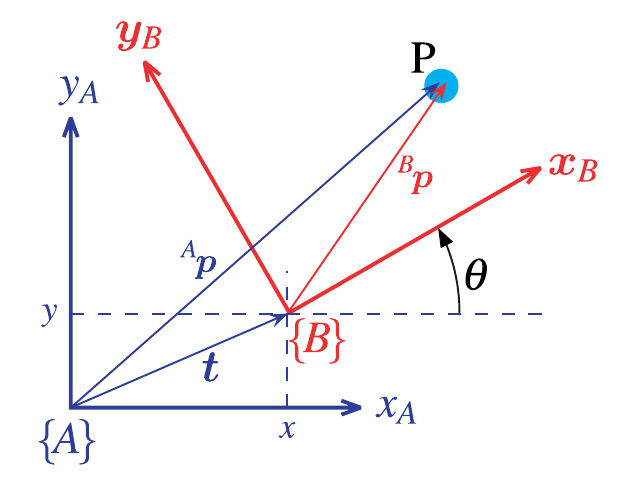
\includegraphics[height=0.5\textheight]{../figures/Corke-fig2.6.png}

\footnotesize Peter Corke \emph{Robotics, vision and control}
\end{center}
\end{frame}

\section{Manipulador como cadena de transfomraciones}
\label{sec:org69df853}

\begin{frame}[label={sec:orgf9a91b6}]{Transformación básica - rotación}
\begin{center}
 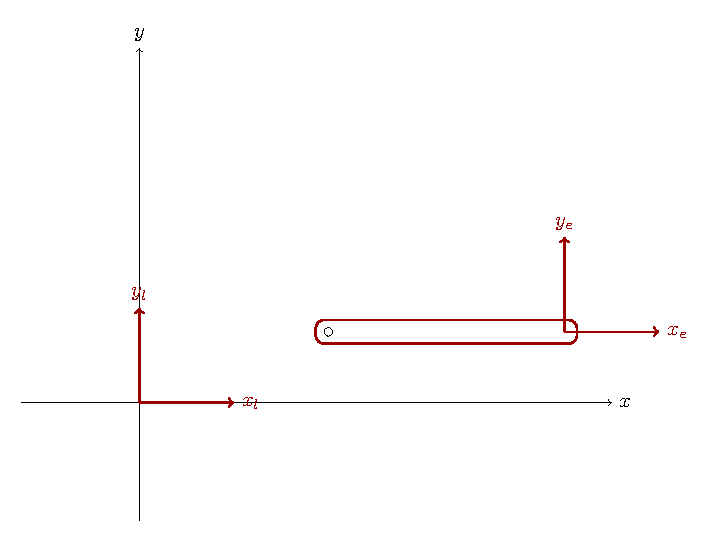
\includegraphics[height=0.8\textheight]{../figures/2d-revolute-default-pos.pdf}
\end{center}
\end{frame}


\begin{frame}[label={sec:org56b8091}]{Transformación básica - rotación}
\begin{center}
 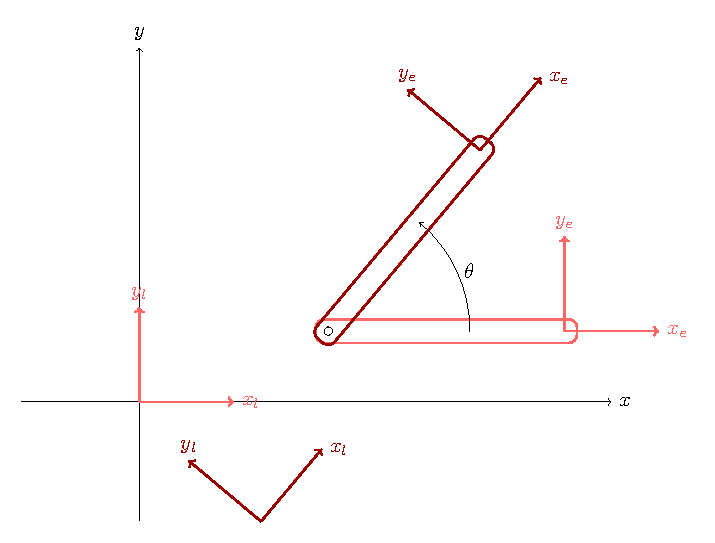
\includegraphics[height=0.8\textheight]{../figures/2d-revolute.pdf}
\end{center}
\end{frame}

\begin{frame}[label={sec:org6fb97ba}]{Transformación básica - desplazamiento}
\begin{center}
 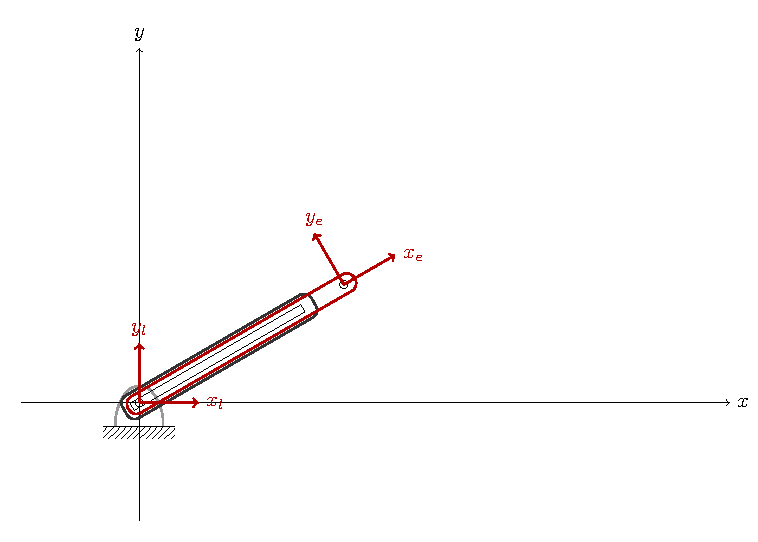
\includegraphics[height=0.8\textheight]{../figures/2d-prismatic-default-pos.pdf}
\end{center}
\end{frame}

\begin{frame}[label={sec:org2324092}]{Transformación básica - desplazamiento}
\begin{center}
 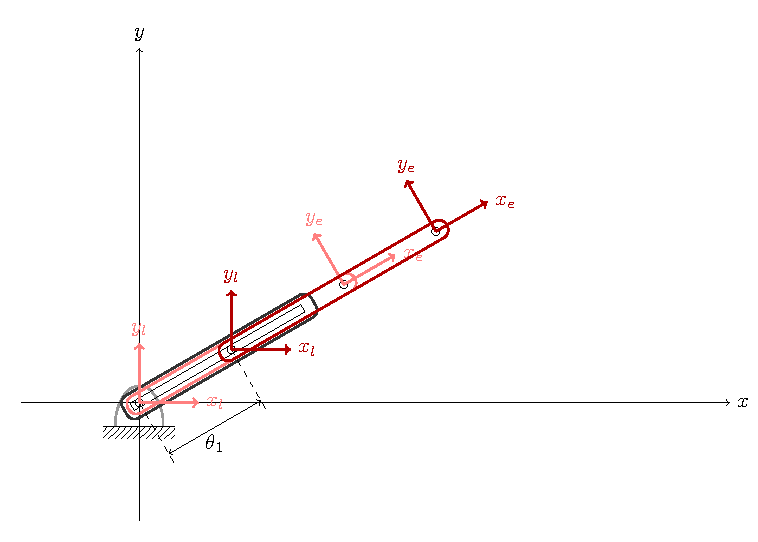
\includegraphics[height=0.8\textheight]{../figures/2d-prismatic.pdf}
\end{center}
\end{frame}
\begin{frame}[label={sec:orgc7ebef5}]{Cadena de transformaciones}
\begin{center}
 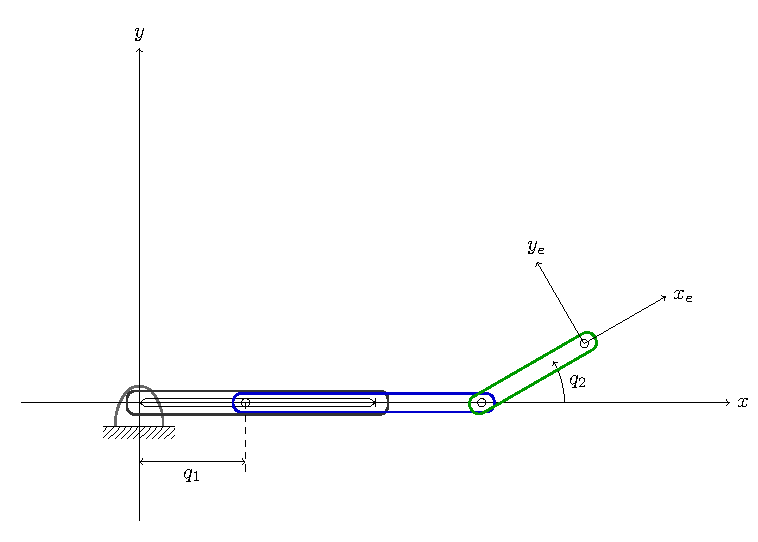
\includegraphics[height=0.8\textheight]{../figures/2d-2dof-prismatic-revolute.pdf}
\end{center}
\end{frame}


\begin{frame}[label={sec:org840dfbd}]{Cadena de transformaciones}
\begin{center}
 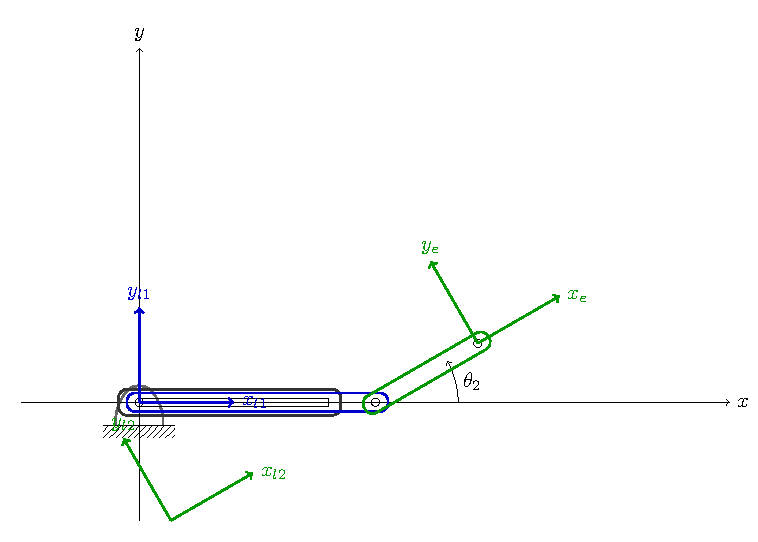
\includegraphics[height=0.8\textheight]{../figures/2d-2dof-prismatic-revolute-prism0.pdf}
\end{center}
\end{frame}

\begin{frame}[label={sec:orga415710}]{Cadena de transformaciones}
\begin{center}
 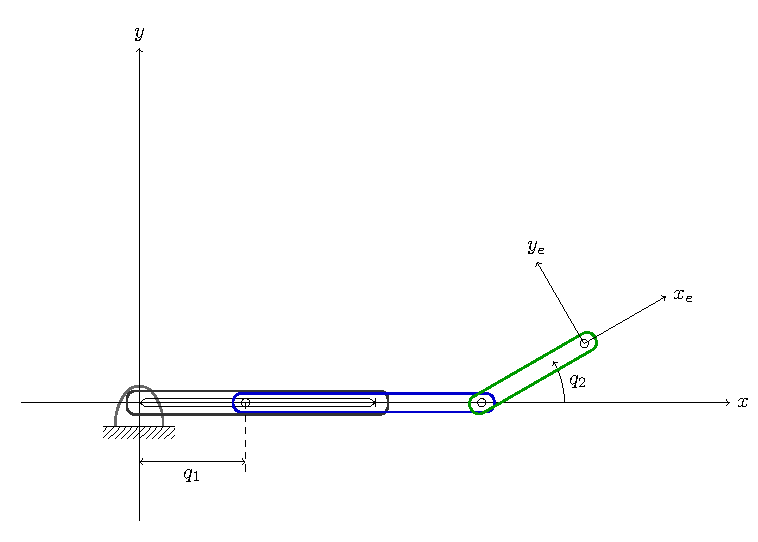
\includegraphics[height=0.8\textheight]{../figures/2d-2dof-prismatic-revolute.pdf}
\end{center}
\end{frame}

\begin{frame}[label={sec:orgd477906}]{Ejercicio - Articulación prismática y articulación revolutaria}
\begin{center}
 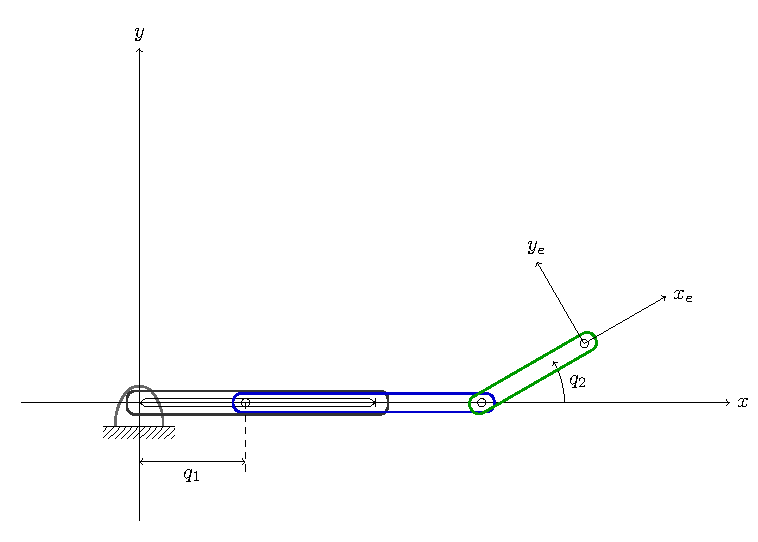
\includegraphics[height=0.8\textheight]{../figures/2d-2dof-prismatic-revolute.pdf}
\end{center}
\end{frame}
\end{document}